\section{Theory of Operations}

The SPI (Serial Peripheral Interface) core is equipped with a variety of features that make it a versatile and efficient choice for synchronous serial communication in embedded systems. These features
are described in-depth in the Register Interface section, but here is a brief overview:

\begin{itemize}
    \item \textbf{Full Duplex, Three-Wire Synchronous Data Transfer:} Enables simultaneous transmission and reception of data, enhancing communication efficiency.
    \item \textbf{Master or Slave Operation:} The SPI core can function as either a master, initiating and controlling communication, or as a slave, responding to the master's commands.
    \item \textbf{LSb First or MSb First Data Transfer:} Flexibly configures the data transmission order based on the system requirements, supporting both Least Significant Bit (LSb) first and Most Significant Bit (MSb) first formats.
    \item \textbf{Programmable Bit Rates:} Allows customization of the SPI clock speed to match the performance needs of different peripherals and system constraints.
    \item \textbf{End of Transmission Interrupt Flag:} Notifies the system when a data transmission cycle is complete, facilitating efficient interrupt-driven communication.
    \item \textbf{Write Collision Protection:} Prevents data corruption by detecting and handling scenarios where multiple write attempts occur simultaneously.
    \item \textbf{Wake-up from Idle Mode:} Supports low-power operations by enabling the SPI core to wake up from idle states upon specific events or triggers.
    \item \textbf{Double-Speed Master SPI Mode:} Increases data throughput by doubling the SPI clock rate in master mode, enhancing overall system performance.
\end{itemize}

% Block Diagram
\begin{figure}[H]
    \centering
    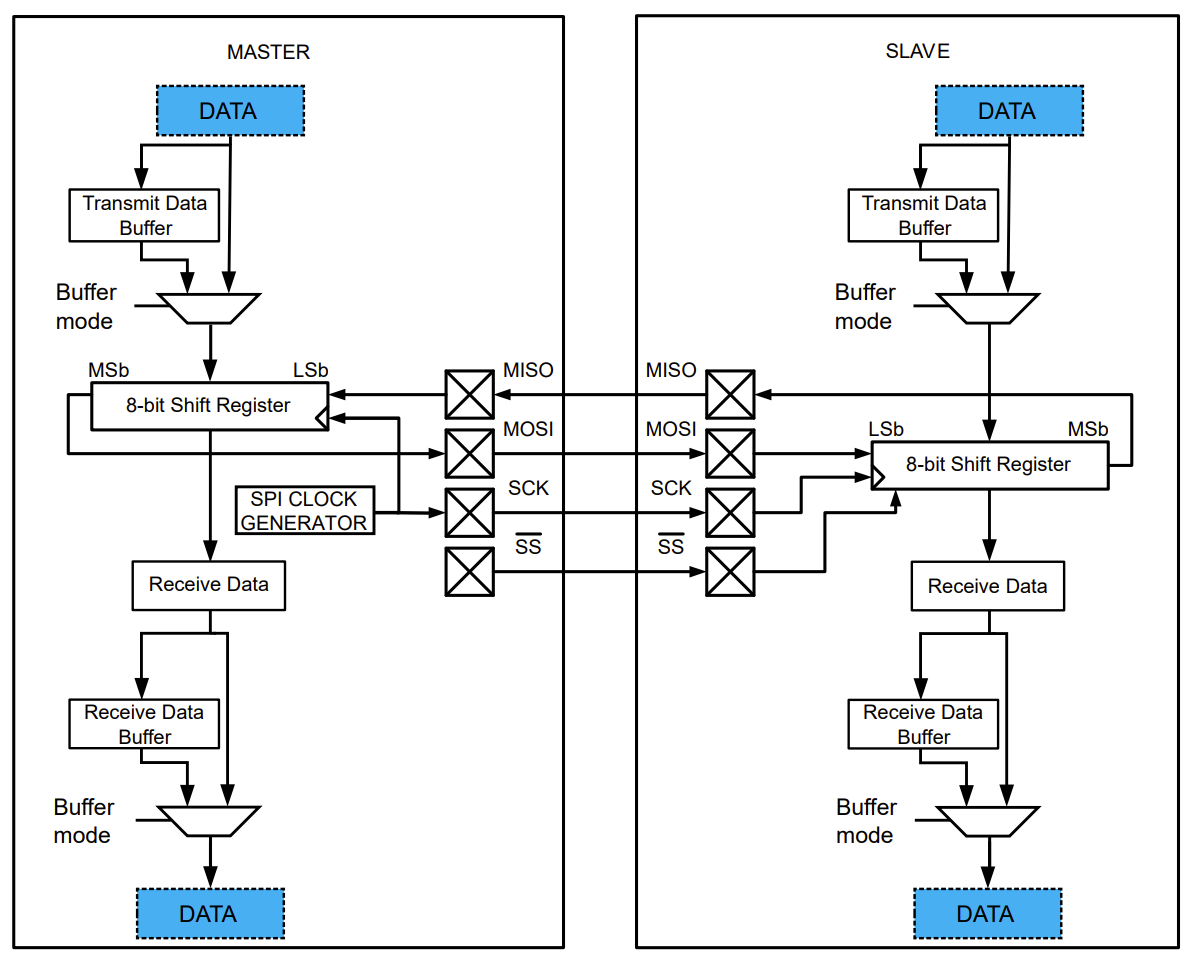
\includegraphics[width=0.8\textwidth]{images/spi_block_diagram.png}
    \caption{SPI Core Block Diagram}
    \label{fig:spi_block_diagram}
\end{figure}

\subsection{Interface Timing}

Spi has a synchronous Apb3 interface, and a Spi interface. The timing diagram shown below
in Figure~\ref{fig:timing} represents an instantiation with the following
parameters.

\begin{lstlisting}[language=Scala]
    val mySpi = new Spi(
      dataWidth = 8, 
      addrWidth = 8 ) 
\end{lstlisting}
    
\begin{figure}[h]
    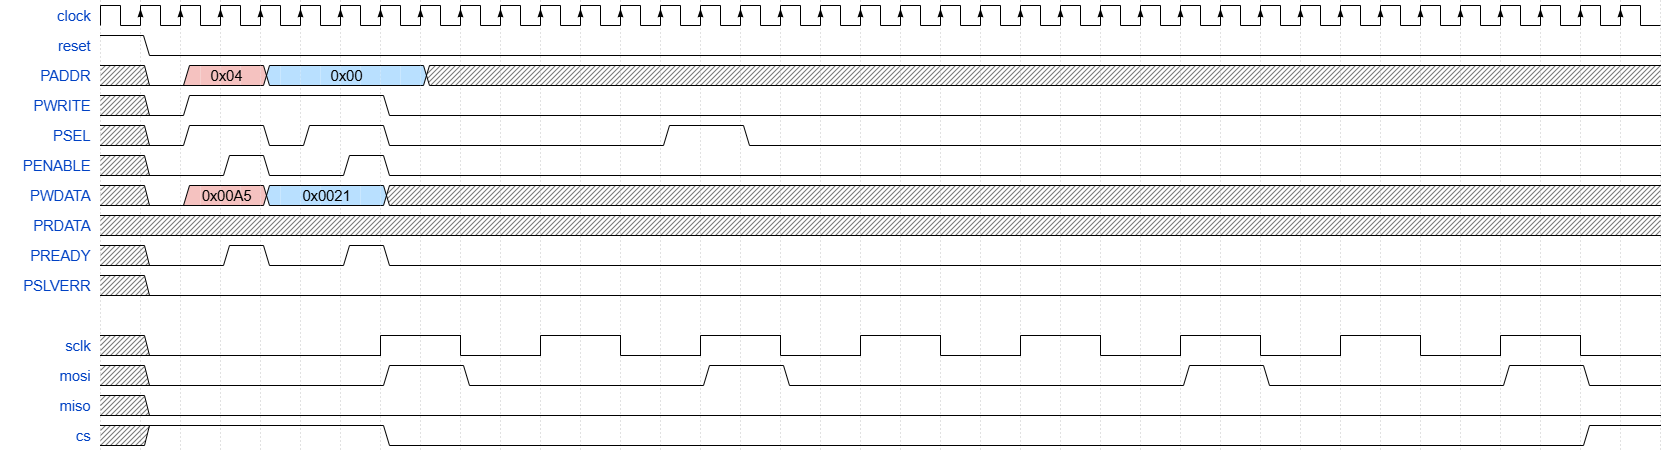
\includegraphics[width=\textwidth]{images/wavedrom.png}
    \caption{Timing Diagram}\label{fig:timing}
  \end{figure}

This shows the operation of enabling the Spi as a Master following the Apb protocol. Register CTRLA is written to configure the Master
as MSB first, prescaler set at 4, and no double clock speed. Since CTRLB is not written to, and its default values are 0, there will be no buffer mode, 
and CPOL/CPHA mode set to 0. The DATA register is written with 0xA5, which is the data the Master will transmit to the Slave. 

The \textit{sclk} port is driven once the master is enabled via CTRLA. Since CPOL/CPHA is set to 0, \textit{sclk} begins low, and sampling happens on the rising edge.
\textit{mosi} shifts out the value written to DATA, one bit at a time, MSB first. \textit{miso} stays low since the Slave is not sending any data to the Master. \textit{cs} 
is driven low once transmission begins, signalling to the Slave that a transaction is occuring.

Once the transaction is complete, all the SPI ports go low. 


